\documentclass{article}
\usepackage[colorlinks=true, allcolors=blue]{hyperref}
\usepackage{graphicx}
\usepackage{tabularx}
\usepackage{amsmath}

\title{Revnets}
\author{Filip\\f@filip.world}

\begin{document}
\maketitle

\begin{abstract}
  Smart contracts have enabled new models for organization and governance, but have in some ways failed to deliver on the promise of truly decentralized coordination. Among other causes, this is often due to the challenge of bootstrapping an organization while creating a product. The centralized nature of this process often leaves the founding team or core developers with little incentive to distribute power by the time a community has been formed. This leaves both parties worse-off: founders must contend with the day-to-day overhead of running a DAO or a governance system which has little to do with their end product, and participants must contend with the risk of misalignment, rugpulls, and scams. \textbf{Revnets} are a new model for creating, scaling, and operating decentralized networks according to pre-defined economic incentives which align participants and remove the need for governance, freeing founders from day-to-day management and making rugpulls impossible.
\end{abstract}

\section{Mechanism}

Each Revnet accepts a specific currency, chosen when the network is created. Anyone can pay a Revnet with its currency to issue the Revnet's tokens, or they can destroy tokens to reclaim currency from the Revnet. For illustrative purposes, this section describes a network which accepts ETH and issues a \$token.\footnote{In practice, Revnets can accept and denominate prices in other currencies. For a clearer understanding of USD-based accounting, see Section~\ref{sec:accounting_types}.}

Under the Revnet's initial conditions, payers receive 1 \$token per ETH. \$token issuance evolves over generations which last a pre-defined length of time (1 day, for example). Three mechanisms determine how \$tokens behave:

\begin{itemize}
  \item The \textbf{Price Ceiling} is the ETH price to create new \$tokens, expanding the \$token supply. The price ceiling increases at a fixed rate each generation, making network expansion more expensive over time.
  \item The \textbf{Price Floor} is the ETH value that can be reclaimed from the network by destroying \$tokens, contracting the \$token supply. The price floor increases dynamically as the network contracts or expands.
  \item The \textbf{Price Window}. Liquidity can be added to a \$token$\leftrightarrow$ETH market\footnote{Our initial implementation uses a Uniswap v3 liquidity pool.} at any time. While the \$token's market price is between the price ceiling and price floor, \$tokens are purchased and sold on the market. Otherwise, purchases and sales are fulfilled at the price ceiling or price floor, expanding or contracting the \$token supply in response to demand.
\end{itemize}

In practice, Revnets issue \$tokens at the price ceiling until a \$token$\leftrightarrow$ETH market forms. From that point onwards, \$tokens are purchased and sold on the market until the price reaches the price ceiling or price floor, at which point the \$token supply will expand or contract to meet market demand.

When somebody pays a Revnet, they have the option to immediately sell or destroy their tokens for a partial refund. Revnets which route ongoing payments from customers to the network allow buyers to choose between receiving a rebate for part of their purchase, or to participate in the future growth of the network.

Revnets can specify a \textbf{boost} which routes a percentage of purchased \$tokens to a specific address called the \textbf{boost operator} for a pre-determined length of time after the network's creation. While the boost is active, the boost operator can route percentages of it to the addresses and Revnets of their choosing, but only up to the pre-defined boost percentage (the operator cannot increase the percentage of tokens being routed to the boost). Revnets also have the option to pre-mint an arbitrary number of \$tokens to the boost operator upon the network's creation. The boost operator could be a core team or developer multisig, but it could also be a staking rewards contract, an airdrop stockpile, or something else. 

Once a Revnet is deployed, all of its parameters are locked in place.

\subsection{Price Ceiling}

The cost to expand the \$token supply increases over time. This is done by reducing the number of \$tokens issued per ETH with each passing generation. This reduction is dictated by a price ceiling function, which compounds at a rate $r_c$ set by the network's creator.

The price ceiling function\footnote{Also see the interactive price ceiling function on \href{https://www.desmos.com/calculator/ey9fhuslwe}{Desmos}} can be expressed as:

\begin{equation}
  T_n = T_1 \cdot (1 - r_c)^{(n - 1)}
\end{equation}

where:
\begin{itemize}
  \item $T_n$ is the number of tokens issued per ETH in the $n^{th}$ generation,
  \item $T_1$ is the number of tokens issued per ETH in the first generation,
  \item $r_c$ is the price ceiling curve, or rate of decrease per generation (expressed as a decimal), and
  \item $n$ is the generation number, which increments sequentially starting from 1.
\end{itemize}

Since Revnets have a $T_1$ (initial price) of 1 \$token per ETH, this can be simplified to:

\begin{equation}
  T_n = (1 - r_c)^{(n - 1)}
\end{equation}

The price ceiling encourages participants to join the network early. The earlier a participant joins, the more \$tokens they receive for their ETH.

\begin{figure}[h]
  \centering
  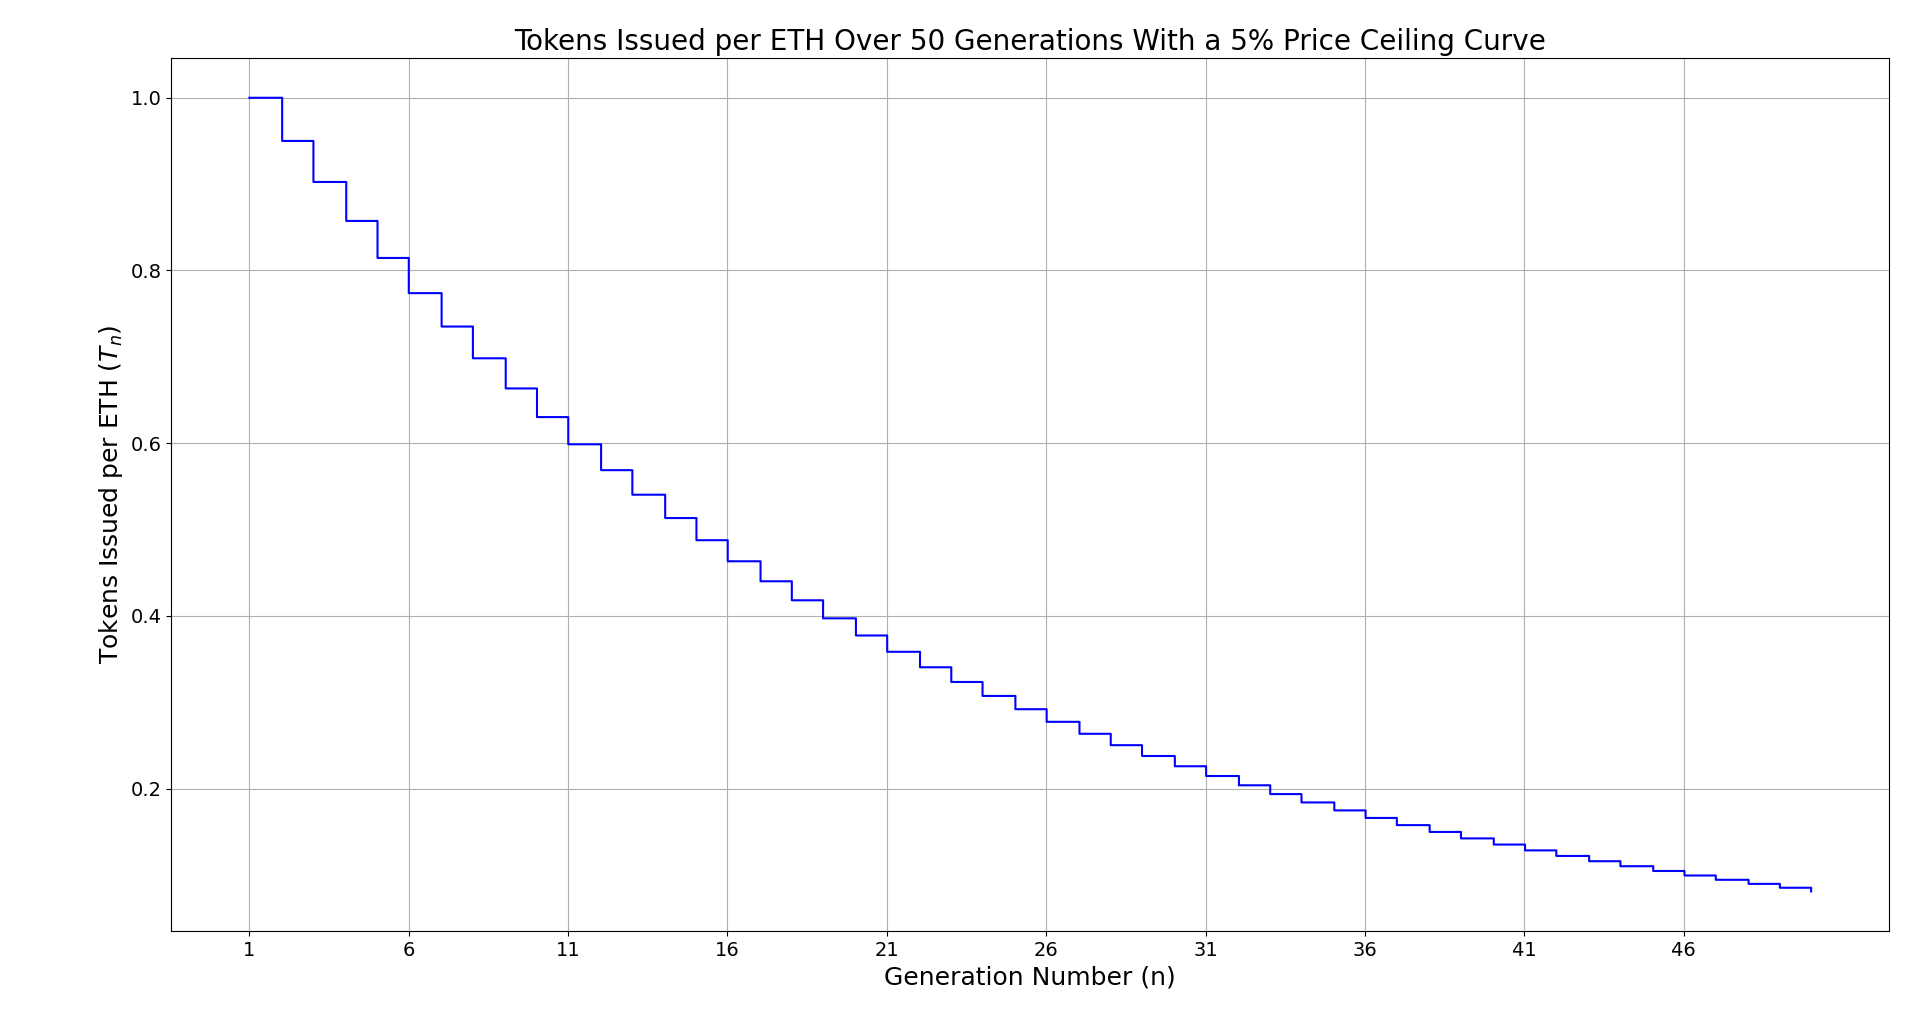
\includegraphics[width=\textwidth]{figures/single-ceiling-curve.png}
   \caption{This figure shows how $T_n$ (the number of \$tokens issued per ETH in the $n^{th}$ generation) varies across 50 generations with a 5\% price ceiling curve $(r_c = 0.05)$. Note that $T_n$ decreases rapidly at first, then more gradually as $T_n$ tends towards 0 over many generations.}
\end{figure}

\clearpage
\begin{figure}[h]
  \centering
  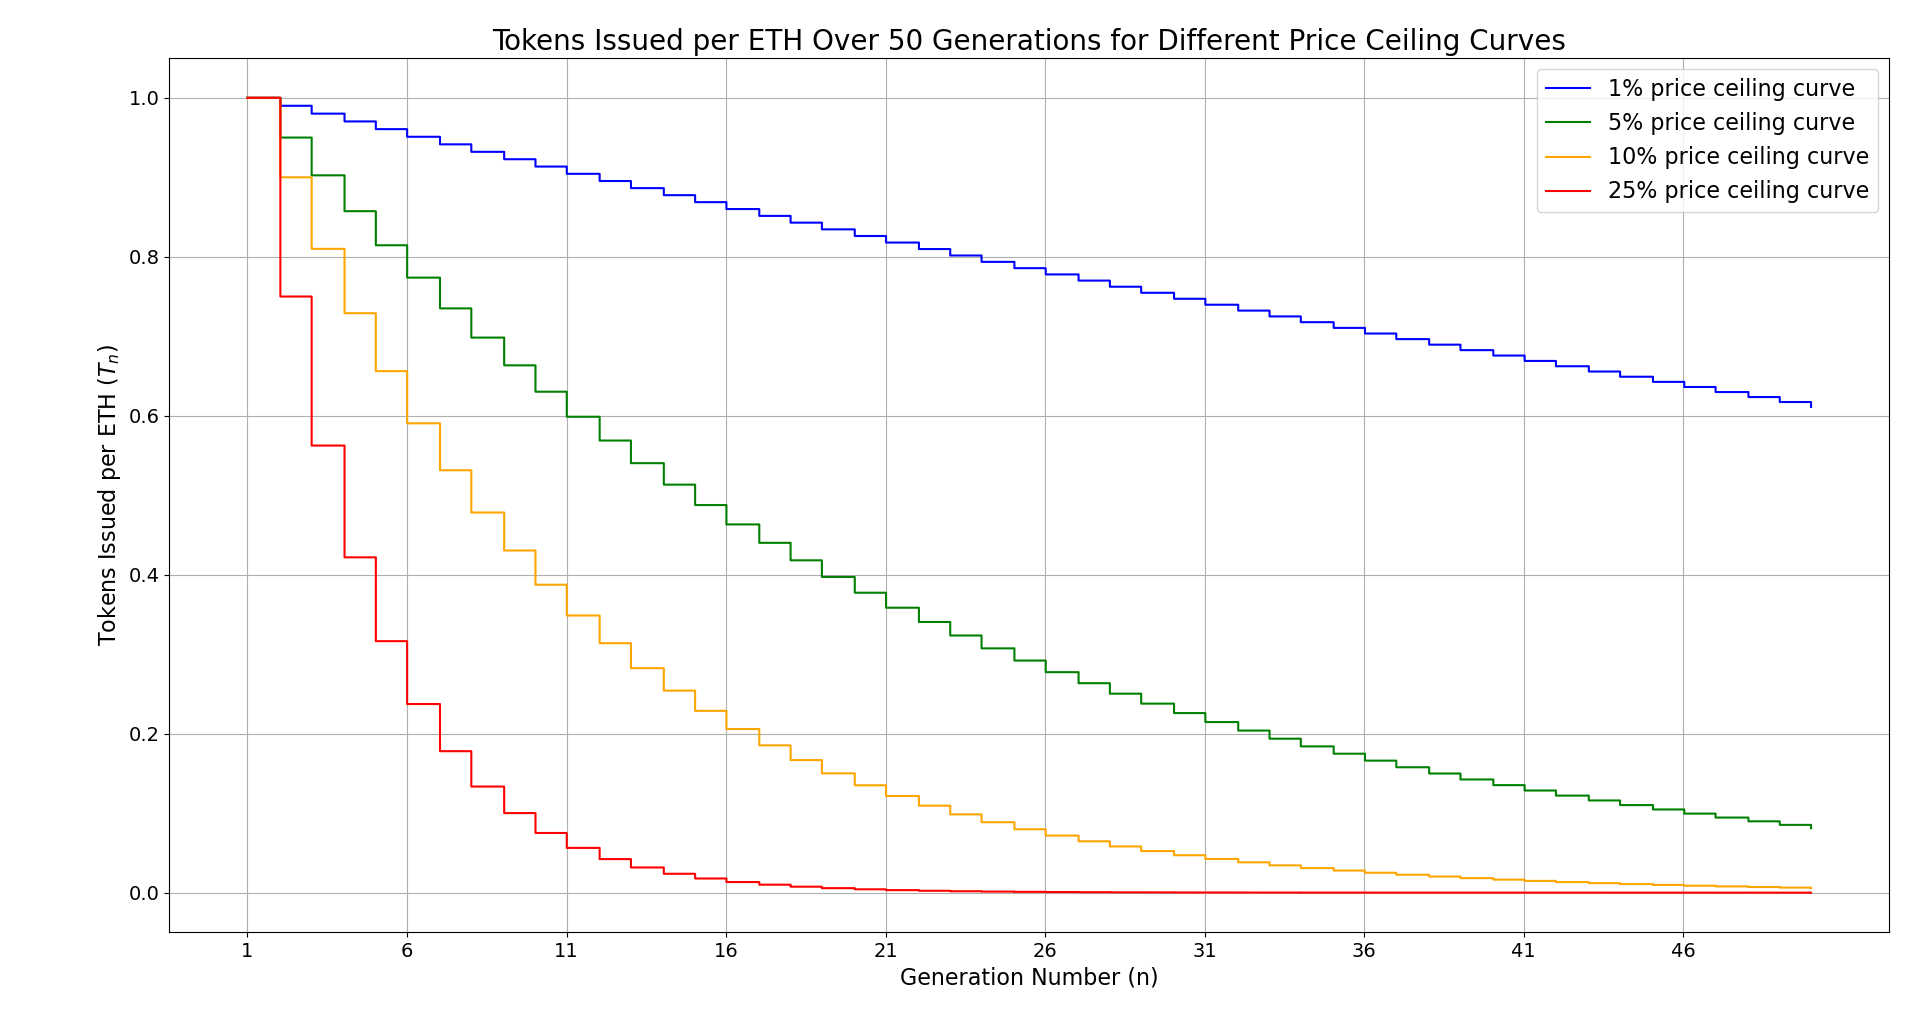
\includegraphics[width=\textwidth]{figures/multi-ceiling-curves.png}
  \caption{This figure shows how $T_n$ varies over 50 generations with 1\%, 5\%, 10\%, and 25\% price ceiling curves $(r_c = 0.01, 0.05, 0.1, 0.25)$. Note that for greater entry curves, $T_n$ tends towards 0 more quickly.}
\end{figure}

\subsection{Price Floor}

Anyone can destroy their \$tokens to reclaim ETH from the network. The amount of ETH they can reclaim is determined by the price floor function, which is dynamically calculated based on a price floor curve $r_f$ set by the network's creator, the total \$token supply, and the amount of ETH in the network.

The price floor function\footnote{Also see the interactive price floor function on \href{https://www.desmos.com/calculator/9pewqesyj5}{Desmos}} can be expressed as:

\begin{equation}
  V_r = \frac{V_t \cdot x}{s}\left(\left(1-r_f\right)+\frac{r_f \cdot x}{s}\right)
\end{equation}

where:
\begin{itemize}
  \item $V_r$ is the amount of ETH which gets reclaimed,
  \item $V_t$ is the total amount of ETH in the network,
  \item $s$ is the total \$token supply,
  \item $r_f$ is the price floor curve (expressed as a decimal), and
  \item $x$ is the number of \$tokens being burned.
\end{itemize}

Unless $r_f$ is 0, this function ensures that as more \$tokens are destroyed (i.e., the larger $x$ is), the more ETH is reclaimed per token.\footnote{If $r_f$ is 0, each \$token will yield the same amount of ETH when destroyed.} This means the first participants to destroy their \$tokens get less ETH per \$token than participants who destroy their \$tokens later. This incentivizes participants to stay in the network longer than other participants in order to increase the amount of ETH they can reclaim.

\begin{figure}[ht]
  \centering
  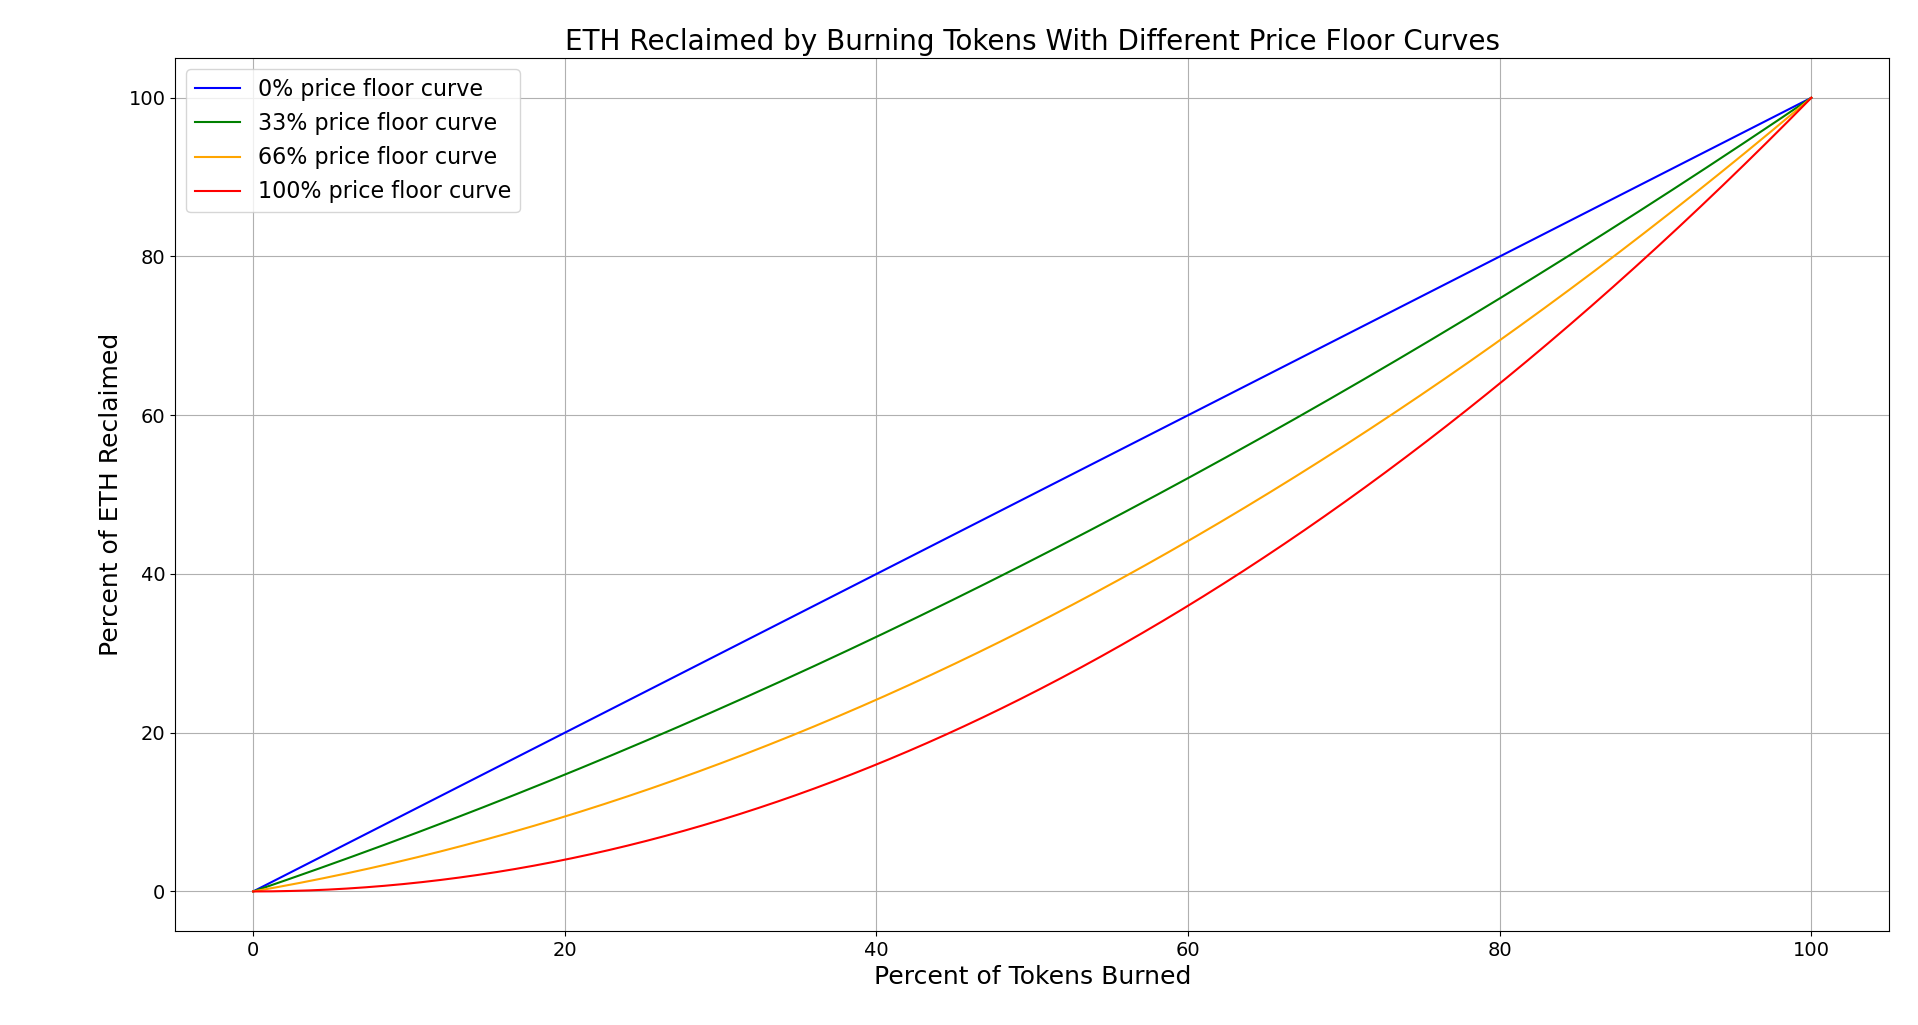
\includegraphics[width=\textwidth]{figures/multi-floor-curves.png}
  \caption{This figure shows price floor functions with price floor curves of 0\%, 33\%, 66\%, and 100\% $(r_f = 0, 0.33, 0.66, 1)$. The $x$ axis represents the percentage of the total \$token supply being destroyed, and the $y$ axis represents the percentage of the network's ETH which is reclaimed. Note that with a 0\% price floor curve $(r_f = 0)$, reclaim amounts are linear with respect to the number of tokens being destroyed---a network participant which destroys \textit{e.g.} 10\% of the total token supply can reclaim 10\% of the network's ETH. The larger the price floor curve, the less ETH earlier reclaimers receive.}
\end{figure}

\section{Applications}

Revnets are particularly beneficial for applications which gain value from network effects, where the value of the service or product increases as more people participate. Revnets are most capable of accomplishing complex coordinated tasks while the boost is active and can be strategically deployed by the boost operator, placing an inherent limitation on the duration and scale of centrally coordinated efforts within a Revnet.

Revnets excel in scenarios where individual contributions, even when isolated, can contribute to the overall project. An anonymous individual can meaningfully contribute to an online encyclopedia or provide reviews for local businesses, making it feasible to coordinate hundreds or thousands of contributors to a project. Revnets are not well-suited to endeavors which require ongoing support from a centralized, hierarchical structure. For instance, a Revnet would struggle to compete with a large-scale manufacturing company or to orchestrate the construction of complex infrastructure projects.

\subsection{Overcoming Existing Network Effects}

Google Maps is popular, but comes with several downsides: it is proprietary, its API is expensive, it has limited offline support, and it lacks data privacy. OpenStreetMap, an open-source alternative, addresses many (if not all) of these concerns, but lacks user-generated reviews and addresses labels. If OpenStreetMap or a project like it were to use a Revnet model with a price ceiling to reward early participants, it might build enough momentum to become viable and eventually compete with proprietary options.

Similarly, alternative social media platforms, such as Mastodon, and protocols like XMPP or Gemini could effectively generate early momentum as Revnets. These Revnets wouldn't necessarily have to monetize the primary product---in line with existing corporate models, they could derive revenue from advertising or the sale of premium services and products, such as web hosting or educational resources. 

Currently, network effects are often overcome by using investor funding to subsidize a product, undercutting competition. Once these products secure a dominant market position, prices are increased, trapping users in a more expensive ecosystem. Revnets provide an alternative to this model, driving the cost per consumer down as the network achieves scale.

\subsection{Governance}

Revnet tokens adhere to the \texttt{ERC20Votes} standard, meaning they can be used in conjunction with governance tools like Snapshot and Governor Bravo for offchain or onchain token voting governance. Importantly, Revnet governance cannot control the allocation of the network's funds, as funds only leave the network according to the Revnet's pre-defined rules. This means Revnets are not subject to a wide range of governance attacks, hostile takeovers, and misaligned incentives which affect DAOs and other governance structures. Revnets are a strong fit for foundations and governing bodies which steward DeFi protocols, software projects, or any other coordinated effort from a distributed community. Revnet mechanisms encourage long-term orientation and distribute tokens accordingly, leading to favorable token distributions and governance outcomes.

\subsection{Gated Networks}

Ethereum wallets offer straightforward sign-in support for web applications, making Revnets a strong fit for token-gated content. A content creator can deploy a Revnet and allow token holders to access exclusive material, and can use token voting to guide the direction of future projects.

This can also be advantageous for token-gated platforms---since participants will have access to the growth of a network, they're more likely to participate in that growth. This is a major advantage for platforms which derive value from their users:

\begin{table}[h]
  \centering
  \begin{tabularx}{\textwidth}{|X|X|}
    \hline \textbf{Category} & \textbf{Examples} \\
    \hline Traditional social media. & Twitter, Instagram, and Facebook. \\
    \hline Forums and real-time chat services. & Reddit, Discord, and IRC. \\
    \hline Content creation and streaming services. & YouTube, Soundcloud, and Twitch. \\
    \hline Review and rating platforms. & Yelp, TripAdvisor, and Rotten Tomatoes. \\
    \hline News and Blogging platforms. & Medium, Mirror, and Tumblr. \\
    \hline Open or volunteer research and science. & Folding@home, BOINC, and LHC@home. \\
    \hline DeFi platforms which rely on user liquidity. & Uniswap, Compound, and Stargate. \\
    \hline
  \end{tabularx}
\end{table}

All else being equal, users are more likely to put value into a platform which allows them to receive a portion of future growth over one which doesn't. Community ownership also prevents the platform from switching to a more extractive business model once it achieves scale, which is a frequent misalignment between users and platforms.

\section{Contract Implementation}

Revnets are implemented as Solidity smart contracts, and are intended for use on Ethereum, Ethereum L2s, and other environments with Solidity support. Revnets are built on top of and extend the Juicebox\footnote{See the \href{https://docs.juicebox.money}{Juicebox Docs}.} protocol. Revnets leverage Juicebox's discount rate logic for price ceiling calculations, its redemption logic for price floor calculations, and its reserved rate logic for boost calculations.

While the price of a Revnet's token is between the price ceiling and the price floor, payments are routed to a Uniswap v3 liquidity pool by a Buyback Delegate\footnote{See the Buyback Delegate contracts on \href{https://github.com/jbx-protocol/juice-buyback}{GitHub}.} contract if possible. The Buyback Delegate contract routes incoming payments to the Uniswap pool if doing so would yield more tokens than a payment into the network would create.

Each Revnet is a Juicebox project, which is deployed, owned, and administered by a deployer contract. Our initial implementation includes a basic deployer, a deployer which adds pay delegates\footnote{See the \href{https://docs.juicebox.money/dev/learn/glossary/delegate/}{delegate documentation}.} to be called when the Revnet is paid, and a deployer which allows the Revnet to mint tiered ERC-721 NFTs when people pay it. These deployers are available on \href{https://github.com/mejango/retailism-templates}{GitHub}.

\subsection{Accounting Types}\label{sec:accounting_types}

If the network uses USD-based accounting, payers will receive 1 token per USD worth of ETH under the network's intial conditions. For instance, if the ETH price is 1,000 USD, paying 1 ETH into the network will yield 1,000 tokens.

\subsection{L2s}

\end{document}

